\chapter{Introducción}
\label{cap:introduccion}

\section{Antecedentes y motivación}
\label{intro:motivacion}

Los desastres naturales en Chile han sido frecuentes en los últimos años. Sólo por mencionar algunos de los más recientes: la erupción del volcán Chaitén (Mayo, 2008), el terremoto en Tocopilla (Noviembre, 2007), el terremoto en Concepción (2010), el incendio de las Torres del Paine (Diciembre, 2011), el incendio en Valparaíso (Abril, 2014), la erupción del volcán Villarrica (Marzo, 2015), los aluviones en el norte (Marzo, 2015), entre otros. Dependiendo de las características de la emergencia, surgen en la población diversos tipos de necesidades: alimentos, agua, luz eléctrica, refugio, rescate o comunicación, entre otras. Muchas veces éstas pueden no ser detectadas por las autoridades; al menos, no de forma expedita, lo que resulta perjudicial para las personas que intentan sobrellevar la crisis de la mejor manera posible, cuando se ve involucrada una necesidad básica, como la falta de agua, donde la vida de los afectados puede verse comprometida. El problema anteriormente descrito, no es sólo para las autoridades; \citep{ChatoSurvey}, señalan que el comportamiento humano ante crisis como éstas, no es quedarse esperando por ayuda o huir en pánico, sino de intentar tomar decisiones rápidas en base a la información que conocen. Esto quiere decir que existe gente dispuesta a ayudar, aun siendo ellos mismos los afectados; pero no siempre disponen de la información necesaria para saber hacia dónde apuntar sus esfuerzos. Resulta útil, dado todo lo anterior, tener algún medio que concentre las necesidades que pueda tener una población dentro del país, para acudir en su auxilio dada la ocurrencia de una emergencia catastrófica, como las mencionadas. Para ello la concentración de estas necesidades se ha de realizar tan pronto como sean emitidas, es decir, deben detectarse en tiempo real.

Los académicos del proyecto FONDEF IDeA (Dos etapas), código ID15I10560 de la Universidad de Santiago de Chile, están trabajando en el desarrollo de una plataforma de procesamiento de flujo de datos generados en contextos de desastres; se busca proveer la infraestructura necesaria para la generación de herramientas capaces de apoyar la toma de decisiones en escenarios de desastres. Esta plataforma hace uso de la información generada por los usuarios en redes sociales como fuente de datos. Para realizar la prueba de concepto de la plataforma se planea desarrollar tres aplicaciones base, orientadas a facilitar la coordinación de voluntarios, detección de necesidades y difusión de información de interés.

En este trabajo, en particular, se ataca el problema de la detección de necesidades de la población y apoyar el desarrollo de la plataforma de \textit{streaming}, en relación a qué operadores se han de construir y cómo ha de estructurarse el sistema para operar sobre datos a nivel nacional.

\section{Descripción del problema}
\label{intro:problema}

El problema que aborda esta memoria, es el hacer uso de la información generada por la población por medio de \textit{Twitter} para que, en caso de alguna emergencia de carácter nacional, pueda prestarse apoyo en tiempo real a las autoridades encargadas de la toma de decisiones; por ejemplo, dándoles a conocer en qué lugar exactamente se requiere asistir a la población con un determinado tipo de ayuda, según la necesidad que se presente. ¿Cómo detectar y localizar en tiempo real las necesidades expresadas por la población en redes sociales basadas en texto de manera de generar una nueva fuente de datos para mejorar la toma de decisiones?

\section{Solución propuesta}
\label{intro:solucion}

Se propone un sistema capaz de recolectar y analizar de manera automática los eventos generados en la red social \textit{Twitter} en tiempo real, de manera que, al ocurrir un escenario de desastre, determine si la publicación expresa una necesidad y, en caso de que así sea, determine su posición geográfica. 

La solución propuesta consta de dos partes: por un lado la plataforma y lógica de procesamiento capaz de realizar la labor antes mencionada y, por otro, la visualización de estos datos.

La plataforma de procesamiento consiste en un sistema de procesamiento de \textit{streams}, construido utilizando el sistema de computación distribuida de \textit{Apache Storm}, el cual basa su funcionamiento en transformar el problema en un grafo donde cada vértice representa un nodo que realiza una tarea, pudiendo existir múltiples instancias de cada nodo alojadas en un sistema distribuido, como un \textit{cluster} de computadores. Así, internamente, la plataforma está compuesta de operadores que discriminan cuándo un evento debe ser entregado a la aplicación de visualización para ser mostradao al usuario. Uno de estos operadores permitirá realizar la categorización del texto de entrada por medio un un clasificador bayesiano.

\section{Objetivos y alcance del proyecto}
\label{intro:objetivos}

\subsection{Objetivo general}
	Construir un sistema escalable para la detección de necesidades de la población en tiempo real, para escenarios de desastre natural haciendo uso de \textit{Twitter}.

\subsection{Objetivos específicos}
\begin{enumerate}
\item	Implementar un método encargado de la recolección de tweets generados dentro del territorio nacional haciendo uso de la API pública de Twitter.
\item	Especificar la taxonomía de las necesidades detectadas.
\item	Diseñar e implementar el clasificador de necesidades.
\item	Definir los elementos de procesamiento para la construcción del sistema capaz de trabajar los datos obtenidos a gran escala.
\item	Implementar una arquitectura escalable que soporte la aplicación.
\item	Evaluar la aplicación bajo condiciones de alto tráfico, como es el caso de una emergencia nacional.
\end{enumerate}

\subsection{Alcances}
\label{subsec:alcances}

Se utilizan las publicaciones de \textit{Twitter} para llevar a cabo el procesamiento de la información y no se considera, en el marco de este trabajo, el uso de una red social alternativa, no porque no sea posible, sino que con la finalidad de acotar el problema.

Las necesidades que la aplicación detecta no son una lista exhaustiva de las posibles existentes, sino de un subconjunto que se ha considerado más importante en el equipo de trabajo del proyecto. De esta forma se logra acotar el problema reduciendo la cantidad de categorías y permitir una mayor precisión en la clasificación, entendiendo la precisión como la relación de elementos clasificados correctamente sobre el total.

Se considera, para la construcción del clasificador, un subconjunto de un \textit{dataset} compuesto de cuatro millones de \textit{tweets} recogidos durante y posteriormente al terremoto en Concepción el 27 de Febrero del 2010. Este conjunto de datos ha de ser limpiado previamente, pues contiene \textit{tweets} en idiomas diferentes al idioma objetivo de este trabajo.

El sistema sólo trabaja en la detección con \textit{tweets} que estén en español.

La validación se realiza a partir de \textit{datasets} con \textit{tweets} reales, sin embargo los flujos generados son sintéticos y no obtenidos de manera online desde \textit{Twitter}.

\section{Metodologías y herramientas utilizadas}
\label{intro:metodologia}

\subsection{Metodología}
\label{subsec:MetodologiaDetalle}

Para la realización de este trabajo se utilizan dos metodologías, la primera está enfocada a la búsqueda de información en bases de datos para realizar la construcción del clasificador de texto, mientras que la segunda, una metodología de desarrollo de aplicaciones ágil, está enfocada en la construcción en sí de las aplicaciones, tanto de la plataforma de procesamiento como de la aplicación de visualización. Ambas son definidas a continuación.

\subsubsection*{Programación Extrema}
\label{subsubsec:XP}

La Programación Extrema (\textit{Extreme Programming}, XP desde ahora en adelante), comenzó como un proyecto el 6 de Marzo de 1996. Es uno de los procesos ágiles más populares y ha sido probado exitosamente en compañías e industrias de todos los tamaños, \citep{XP}. Su éxito se debe a que hace especial hincapié en la satisfacción del cliente por sobre la entrega de todo el software posible.

Esta metodología aporta cinco formas esenciales para mejorar el proceso de desarrollo de software: comunicación, simplicidad, retroalimentación, respeto y coraje. Se busca establecer una estrecha comunicación entre el equipo de desarrollo y el cliente apuntando paralelamente a evitar el sobre-diseño, pero no limita la creatividad en el sentido de que el equipo de desarrollo pueda arriesgarse para proponer alguna implementación diferente a la planteada por el cliente. Siempre se puede obtener retroalimentación de modo que los cambios, en caso de ser necesarios, puedan realizarse lo antes posible. 

La metodología originalmente implementa reglas de trabajo, éstas están divididas en cinco áreas. Para la realización de este proyecto no se consideraron estrictamente todas las que señala la metodología, sino se adaptó el proceso a las características del proyecto como tiempo y dificultad asociada, justamente como la metodología señala. Las actividades desarrolladas se presentan a continuación.

\begin{enumerate}
\item Planeación:
	\begin{itemize}
	\item Se escriben Historias de usuario. 
	\item Se divide el proyecto en iteraciones.
	\item Al comienzo de cada iteración se planea cómo será.
	\end{itemize}
\item Manejo:
	\begin{itemize}
	\item Se le da al equipo una área de trabajo.
	\end{itemize}
\item Diseño:
	\begin{itemize}
	\item Simplicidad. El mejor diseño es el más simple.
	\item Se crean \textit{spikes} para reducir el riesgo.
	\item No se agregan funcionalidades antes de tiempo.
	\item Hacer uso de técnicas de \textit{refactoring}, cada vez que sea posible.
	\end{itemize}
\item Implementación:
	\begin{itemize}
	\item El cliente siempre está disponible. 
	\end{itemize}
\item Prueba:
	\begin{itemize}
	\item Todo el código debe tener pruebas unitarias.
	\item Cuando se encuentra un \textit{bug}, se crean pruebas.
	\item Los \textit{test} de aceptación se ejecutan a menudo y sus resultados son publicados.
	\end{itemize}
\end{enumerate}

Estas reglas se fundamentan en los valores que la metodología quiere entregar, estos valores ya fueron mencionados, a continuación pasan a ser detallados:

\begin{itemize}
\item Simplicidad: Se hace lo que se solicitó, pero no más. Esta práctica maximiza el valor entregado dada una fecha límite. Las metas se alcanzan por medio de pequeños pasos para mitigar errores tan pronto ocurran. Se crea algo de lo que se esté orgulloso y se mantiene en el tiempo a costos razonables.
\item Comunicación: Todos son partes de un equipo y se comunican cara a cara a diario. Se trabaja juntos en todo: desde la toma de requerimientos hasta la implementación. Se crea la mejor solución posible al problema.
\item Retroalimentación: Cada iteración es completada seriamente entregando \textit{software} funcional. Se muestra el \textit{software} a menudo y prontamente para luego escuchar y aplicar los cambios solicitados. Se habla del proyecto y se adapta el propio proceso, no al revés.
\item Respeto: Todos dan y reciben el respeto que merecen como miembros del equipo. Todos contribuyen con valor así sea simple entusiasmo. Los desarrolladores respetan la experiencia del cliente y viceversa. 
\item Coraje: Se dice la verdad sobre el progreso y las estimaciones. No se documentan excusas por si se falla, pues se planea tener éxito. Se adapta a los cambio cuando ocurran.
\end{itemize}

El proceso de XP puede ser apreciado en la Figura \ref{fig:procesoXP}.

\begin{figure}[H]
	\centering
	\captionsetup{justification=centering}
	\includegraphics[scale=0.6]{images/flowChartXP.png}
	\caption[Diagrama de flujo de Programación Extrema.]{Diagrama de flujo de Programación Extrema.\\Fuente: \citep{XP}}
	\label{fig:procesoXP}
\end{figure}

\subsubsection*{\textit{Knowledge Discovery in Databases} (KDD)}
\label{subsubsec:kdd}

Metodología de trabajo para la búsqueda de información en bases de datos, es definida por \citep{KDDFayyad} como ``el proceso no trivial de identificar patrones válidos, nuevos, potencialmente útiles y en última instancia comprensible en los datos". Surge de la necesidad de manejar grandes volúmenes de datos e involucra simultaneamente varias disciplinas de investigación tales como el aprendizaje automático, la estadística, inteligencia artificial, sistemas de gestión de bases de datos, sistemas de apoyo a la toma de decisiones, entre otras.

Si bien puede variar en función del usuario usuario, el proceso generalmente considera las siguientes etapas:

\begin{enumerate}
\item Selección de datos: consiste en buscar el objetivo y las herramientas del proceso de minería, identificando los datos que han de ser extraídos, buscando atributos apropiados de entrada y la información de salida para representar la tarea. Esto quiere decir que, primero se debe tener en cuenta lo que se sabe, lo que se quiere obtener y cuáles son los datos que nos facilitarán esa información para poder llegar a la meta, antes de comenzar el proceso como tal.
\item Limpieza de datos: en este paso se limpian los atributos sucios, incluyendo datos incompletos, el ruido y datos inconsistentes. Estos datos, en algunos casos, deben ser eliminados, pues pueden contribuir a un análisis inexacto y resultados incorrectos.
\item Integración de datos:  combina datos de múltiples procedencias incluyendo múltiples bases de datos, que pueden tener diferentes contenidos y formatos.
\item Transformación de datos: consiste en modificaciones sintácticas llevadas a cabo sobre los datos sin que suponga un cambio en la técnica de minería aplicada. Tiene dos caras, por un lado existen ventajas en el sentido de mejorar la interpretación de las reglas descubiertas y reduce el tiempo de ejecución, por el otro puede llevar a la pérdida de información.
\item Reducción de datos: reducción del tamaño de los datos, encontrando características más significativas dependiendo del objetivo del proceso.
\item Minería de datos: consiste en la búsqueda de patrones de interés que puedan expresarse como un modelo o dependencia de los datos. Se ha de especificar un criterio de preferencia para seleccionar un modelo de un conjunto de posibles modelos. Además se ha de especificar la estrategia de búsqueda (algoritmo), a utilizar.
\item Evaluación de los patrones: se identifican patrones interesantes que representan conocimiento utilizando diferentes técnicas incluyendo análisis estadísticos y lenguajes de consulta.
\item Interpretación de resultados: Consiste en entender resultados de análisis y sus implicaciones y puede llevar a regresar a algunos pasos anteriores.
\end{enumerate}

La representacíón del proceso descrito por la metodología KDD es presentada en la Figura \ref{fig:procesoKDD}.

\begin{figure}[H]
	\centering
	\captionsetup{justification=centering}
	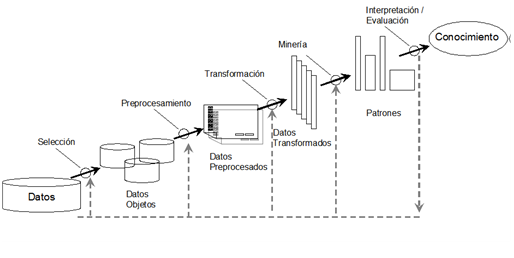
\includegraphics[scale=1]{images/kdd.png}
	\caption[Proceso para el manejo y tratamiento de datos según la metodología KDD.]{Proceso para el manejo y tratamiento de datos según la metodología KDD.\\Fuente: \citep{KDDFigure}}
	\label{fig:procesoKDD}
\end{figure}

\subsection{Herramientas de desarrollo}
\label{subsec:HerrDesarrollo}

A continuación se presentan las herramientas, tanto de \textit{software} como de \textit{hardware} utilizadas para la contrucción del sistema de detección de necesidades.

Se han utilizado diversas herramientas de software para la construcción de la aplicación, éstas son descritas a continuación haciendo especial énfasis en aquellas de gran importancia dentro del desarrollo del proyecto

\begin{itemize}
\item Apache Storm: sistema de procesamiento distribuido que basa su procesamiento en dividir el problema en nodos de un grafo dirigido. Permite el procesamiento de eventos en tiempo real.
\item MongoDB: sistema de gestión de bases de datos no-SQL capaz de lidiar con altas tasas de tráfico y respuestas rápidas para aplicaciones en tiempo real.
\item Mallet: biblioteca de Java que contiene herramientas para el procesamiento de lenguaje natural, clasificación de documentos, extracción de información y otras herramientas de aprendizaje automático sobre texto. 
\item Play Framework: \textit{framework} para aplicaciones tanto Java como Scala, utiliza el modelo de arquitectura de diseño modelo-vista-controlador. Está orientado a la construcción de aplicaciones REST y hace hincapié en la productividad de los desarrolladores.
\end{itemize}

Además de las anteriores, se utilizan herramientas comunes para el desarrollo de proyectos de \textit{software} descritas a continuación:

\begin{itemize}
\item NetBeans (8.1), como herramienta de apoyo a la construcción de la aplicación. Cuenta con licencia GNU.
\item Sublime Text 3 (Build 3103), como editor de textos. El cual requiere de una licencia de pago para su uso.
\item MiKTex (XeLaTeX), producto de software libre, utilizado para la escritura de la memoria. De código abierto.
\item PowerDesigner 16, para la elaboración de diagramas. Su uso requiere de una licencia de pago.
\item Bitbucket (Git), como repositorio y sistema de control de versiones de todo lo referente al proyecto (detector de necesidades, visualizador y documento de memoria). Cuenta con versiones de pago para equipos grandes y gratis para pequeños grupos de desarrollo.
\item Trello (Online), como tablero Kanban para mantener el estado de avance del proyecto. Se utiliza cuenta gratuita.
\item YourKit 1.8.0\_92 64 bits, para evaluación de \textit{performance} de la aplicación. Herramienta de pago, otorga un periodo de evaluación.
\item Windows 10 Home Edition (x64), sistema operativo. Licencia de estudiante.
\item Linux Mint 17.3 (x86), sistema operativo. Licencia GLP.
\item Oracle VirtualBox (5.0.14), utilizado para ejecutar la máquina virtual de Linux sobre Windows. Licencia privativa.
\end{itemize}

\subsubsection*{Herramientas de \textit{hardware}}
\label{subsubsec:HerrHardw}

Se hace uso del equipo del autor de este trabajo cuyas características técnicas son descritas a continuación:
\begin{itemize}
\item Procesador Intel Core i5 2.2 Ghz.
\item 8 GB de memoria RAM.
\item 1 TB de disco duro.
\end{itemize}

\section{Organización del documento}
\label{intro:organizacion}

El resto del documento se organiza de la siguiente manera:

El Capítulo \ref{cap:MarcTeorico}, presenta el marco teórico que sustenta la solución implementada y un análisis del estado del arte en términos de las herramientas y técnicas que han sido utilizadas para dar solucion a problemas similares.

El Capítulo \ref{cap:Requerimientos} describe el proceso de toma de requerimientos de la aplicación. Para ello, siguiendo la metodología XP, se describen de historias de usuario y sus correspondientes criterios de aceptación.

El Capítulo \ref{cap:Diseno}, presenta la arquitectura del sistema y las decisiones que llevaron a que se seleccionase ésta, además, describir la implementación de las aplicaciones visualizador y detector de necesidades, incluyendo los elementos que las componen y, en el caso de esta última aplicación, el porqué del uso de una topología en particular.

El Capítulo \ref{cap:experimentos}, presenta los resultados de la construcción del sistema y evalúa el nivel de replicación de los operadores del sistema y su rendimiento en una simulación de una situación real como fue el terremoto de Concepción en febrero del año 2010.

Finalmente el Capítulo \ref{cap:conclusiones}, presenta las conclusiones del trabajo realizado, el cumplimiento de objetivos tanto general como específicos, los resultados de los experimentos y trabajo futuro.